\section*{\fs{12}Tablica Lekarstwa}
\par{
\fs{12}

\begin{figure}[h!]
    \centering
   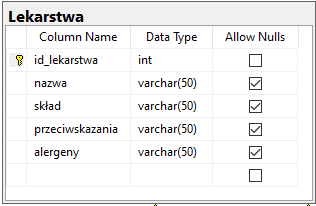
\includegraphics{Images/Zadanie2/Lekarstwa.png}
    \caption{Tablica Lekarstwa}
    \label{fig:my_label}
\end{figure}
\listsinglespacing{
\fs{12}
\begin{lstlisting}[frame=single,language=SQL,]
Select * from Lekarstwa

\end{lstlisting}
\begin{figure}[h!]
    \centering
   \scalebox{.85}{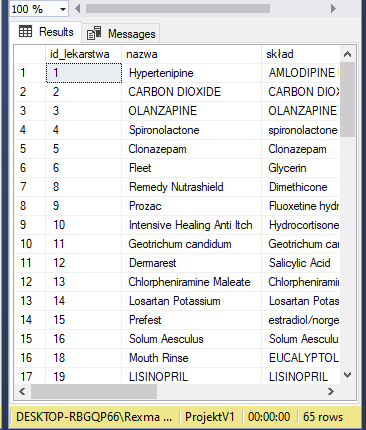
\includegraphics{Images/Zadanie2/Zapelnione/Lekarstwa_query.png}}
    \caption{Wynik Zapytania}
    \label{fig:my_label}
\end{figure}
}